% STS-format research report sample.
\documentclass[11pt,letterpaper]{article}
\usepackage[utf8]{inputenc}
\usepackage[T1]{fontenc}
\usepackage{amsmath,amssymb,amsthm,mathtools}
\let\Bbbk\relax \let\openbox\relax
\usepackage{newtxtext,newtxmath}
\usepackage[margin=1in]{geometry}
\usepackage{microtype,booktabs,array,setspace,fancyhdr,url,tikz}
\usepackage[hidelinks,hypertexnames=false,bookmarks=false]{hyperref}
\microtypesetup{protrusion=false,expansion=false}
\onehalfspacing
\setdisplayskipstretch{1}
\AtBeginDocument{%
  \setlength{\abovedisplayskip}{7pt plus 2pt minus 1pt}%
  \setlength{\belowdisplayskip}{7pt plus 2pt minus 1pt}%
  \setlength{\abovedisplayshortskip}{0pt plus 2pt}%
  \setlength{\belowdisplayshortskip}{7pt plus 2pt minus 1pt}}
\makeatletter
\renewcommand\section{\@startsection{section}{1}{\z@}%
  {-2ex plus -.5ex minus -.2ex}{1ex plus .2ex}%
  {\normalfont\Large\bfseries}}
\renewcommand\subsection{\@startsection{subsection}{2}{\z@}%
  {-1.5ex plus -.3ex minus -.2ex}{.7ex plus .2ex}%
  {\normalfont\large\bfseries}}
\makeatother
\setlength{\emergencystretch}{3em}
\setlength{\parskip}{0pt}
\allowdisplaybreaks
\pagestyle{empty}
\fancyhf{}
\fancyfoot[R]{\thepage}
\renewcommand{\headrulewidth}{0pt}
\fancypagestyle{plain}{\fancyhf{}\fancyfoot[R]{\thepage}\renewcommand{\headrulewidth}{0pt}}
\newtheorem{theorem}{Theorem}[section]
\newtheorem{lemma}[theorem]{Lemma}
\newtheorem{proposition}[theorem]{Proposition}
\newtheorem{corollary}[theorem]{Corollary}
\newcommand{\F}{\mathbb F}
\newcommand{\che}{\chi}
\newcommand{\turnR}{\mathrm R}
\newcommand{\turnL}{\mathrm L}
\newcommand{\Z}{\mathbb Z}
\newcommand{\graphiccredit}[1]{\par\noindent #1\par\medskip}
\begin{document}
\begin{titlepage}
\centering
\vspace*{.8in}
{\LARGE Finite-Support Periodic Highways of Langton's Ant\par}
\vspace{.4in}
{\Large Research Report Sample\par}
\vspace{.6in}
{\large Project researcher: Atharva Jillhewar\par}
\vfill
Research evidence through 12 October 2026\\
Sample revised 12 October 2026\par
\end{titlepage}
\clearpage
\thispagestyle{empty}
\section*{Abstract}
A repeating turn word defines a highway of Langton's ant only if visits
from successive copies request compatible colours at each physical cell.
A necessary and sufficient finite test checks this compatibility and
constructs a finite black seed for every word that passes. Starting from
the least seed, each period-boundary state consists of the translated
seed and disjoint layers of accumulated wake. For a heading-resetting word of length $N$ and nonzero displacement
$d$, stable cell chronology identifies the black-count increase $g$ with
the number of odd translation classes. Conservation then gives
$g\ge2\|d\|_\infty$. Analytic drift exclusions and a symbolic
computer-assisted primitive-diagonal argument, with no period cutoff,
imply $g\in4\mathbb Z_{\ge2}$. For diagonal drift, geometric rigidity
and finite strip certificates force transverse width $W\ge10$.
An explicit period-$104$, growth-$12$ word with an eleven-cell seed
attains that width. First-entry cycles and integer detour charges yield
$N\ge6\|d\|_\infty+2\|d\|_1$, sharpened to $N\ge10m+4$
for $d=(m,-m)$, $m>0$. Routing and incidence identities, polynomial charges and black lifetimes
give further constraints. Formal count walks still require physical
colour consistency. Archived exhaustive
searches exclude all nonzero-drift periods through $48$ and growth-eight
periods through $60$. The computational premises are stated explicitly. All ten growth-eight
drift orbits retain open cases, and eventual highway entry from every
finite seed remains unproved.
\clearpage
\pagenumbering{arabic}
\pagestyle{fancy}
\section{Research question and exact framework}
Langton's ant turns right on a white cell and left on a black cell.
It then flips the cell and moves one unit in its new heading \cite{Langton1986}.
The initial black set is finite. The familiar all-white trajectory develops
a period-$104$ highway, but universal entrance into that highway remains
open. Unboundedness \cite{BunimovichTroubetzkoy1992}, checkerboard routing
\cite{GaleProppSutnerTroubetzkoy1995}, universality on suitable infinite
backgrounds \cite{GajardoMoreiraGoles2002}, and symbolic trace descriptions
\cite{Gajardo2003symbolic} do not settle the finite-seed question.
Related highway and confinement work supplies context
\cite{GajardoLutfallaRao2024,Lutfalla2025sideways,Etse2026confined}.

Which finite turn words can repeat indefinitely from a finite black seed,
and what restrictions follow on growth, drift, width and period? Copies
of a word can revisit a cell in a different phase order. The criterion
below checks their colour requirements in physical order, then uses
that stable chronology to derive the restrictions.
Unboundedness and checkerboard routing are established results. The
criterion and its consequences are developed here, with proof sources
and executable evidence identified in the accompanying archive \cite{Repo}.

Write a state as $(B,p,q)$, with finite $B\subset\Z^2$, position $p$, and
heading $q\in\Z/4\Z$, with $0=N,1=E,2=S,3=W$ and unit vectors
$(u_0,u_1,u_2,u_3)=((0,1),(1,0),(0,-1),(-1,0))$. A
step with turn sign $r=1$ on white and $r=-1$ on black is
\[
(B,p,q)\longmapsto(B\mathbin\triangle\{p\},p+u_{q+r},q+r).
\]
A word $w_0\cdots w_{N-1}$ induces positions $p_0,\ldots,p_N$.
Require heading reset and nonzero drift $d=p_N-p_0=(a,b)$, and put
$g=\#R-\#L$. Each right turn adds one black cell and each left turn
removes one, so $g$ is the black-count increase per period. The period
need not be minimal. Translation and cyclic phase changes are allowed,
as are quarter-turn rotations. Reflection changes chirality and is excluded.
A periodic highway is a finite-seed orbit whose turn trace eventually
repeats such a heading-resetting word with nonzero drift.

\paragraph{Principal results and proof route.}
Theorem~\ref{thm:criterion} decides a proposed word and constructs its seed.
Wake chronology gives the growth--drift bound (Theorem~\ref{thm:density}).
Geometry and strip certificates give diagonal width $W\ge10$
(Theorem~\ref{thm:width}), attained by the explicit example. This width
bound also supports the primitive growth-four exclusion; together the
exclusions in Section~\ref{sec:growthfour} give $g\ge8$. Selected cycles
bound period (Theorem~\ref{thm:period}), sharpened to $N\ge10m+4$
for drift $(m,-m)$. Other identities give necessary conditions. The exhaustive searches
exclude only the finite ranges stated.

\begin{lemma}[Elementary invariants]\label{lem:elementary}
The quantities $q_t-|B_t|\pmod4$ and
$q_t-(p_{t,x}+p_{t,y})\pmod2$ are constant. At each physical cell the
arrival axis is fixed and the turns alternate.
\end{lemma}
Checkerboard routing is classical \cite{GaleProppSutnerTroubetzkoy1995};
the proof fixes this report's conventions.
\begin{proof}
Heading and black count both change by $r_t$ modulo four. Heading parity
and position checker parity both flip each step. Thus every visit to a
fixed cell has the same heading parity, giving its fixed horizontal or
vertical arrival axis. Flipping that cell after each visit forces its
successive colours, and therefore turns, to alternate.
\end{proof}
Heading reset gives $g\equiv0\pmod4$, hence even $N$ and even $a+b$.
The $N/2$ horizontal and $N/2$ vertical steps also give
$a\equiv b\equiv N/2\pmod2$.


The update is reversible: from the new pose, step backward in its current
heading, flip that previous cell, and undo the uniquely determined turn.
A clean translator satisfies $B_N=B_0+d$, with position translated by
$d$ and heading reset. Reversibility extends this whole-state translation to negative times.
It gives no periodicity conclusion for a general finite seed.

Unboundedness has a geometric proof \cite{BunimovichTroubetzkoy1992}.
Let $S_\infty$ be the infinitely visited cells. Two adjacent neighbours
of a recurrent cell cannot both lie outside $S_\infty$: after their last
visits, only one arrival arc remains, but alternating turns require both
outgoing arcs. A bounded orbit would have finite nonempty $S_\infty$;
its $x+y$-maximizer violates this condition. In a finite-height recurrent
strip, each top-level cell similarly forces both horizontal neighbours
recurrent, hence a bi-infinite row. Ruling out such rows requires more
than unboundedness.

\section{A constructive finite test for periodic realisability}
Group the phases by $i\sim j$ when $p_i-p_j\in\Z d$. For a class $I$,
choose $b_I$ and integers $a_i$ with $p_i=b_I+a_i d$. At the physical cell $b_I+nd$, phase $i$ has visit time $i+N(n-a_i)$
when $n\ge a_i$. Order those visits by time and call the resulting
symbol sequence $S_{I,n}$.

\begin{theorem}[Exact criterion]\label{thm:criterion}
The repeated word $w^\omega$ is realisable from a finite black seed if
and only if every $S_{I,n}$ alternates and each stabilised class word
begins with R. It suffices to check
$\min_{i\in I}a_i\le n\le\max_{i\in I}a_i$. A seed is
\[
B=\{b_I+nd:\min a_i\le n<\max a_i,\ S_{I,n}\hbox{ begins with L}\}.
\]
\end{theorem}
\begin{proof}
Phase $i$ in period $k\ge0$ visits $b_I+nd$ exactly when $k=n-a_i$,
giving the stated chronology. Cell flips force alternation. For
$n\ge\max a_i$, the order is independent of $n$; finite support forces
this common first turn to be R, since infinitely many such cells are white.
Conversely, the displayed seed assigns each boundary cell its required
first colour. All stabilised cells start white; alternation then supplies
every later requested colour. Induction on time reproduces the proposed
word, with heading reset and translation by $d$ after each period.
\end{proof}
Sort by decreasing $a_i$, breaking ties by phase. Every boundary word
is a suffix of the stabilised word and inherits its alternation.

\begin{corollary}[Least seed for a fixed trace]\label{cor:leastseed}
Fix an accepted trace starting at time zero, and let $V=\bigcup_i(p_i+\Z_{\ge0}d)$.
Every finite realising seed is $B\sqcup F$ with finite $F\subseteq\Z^2\setminus V$.
Consequently $B$ is the unique least seed. If a class has ordered levels
$a_1\ge\cdots\ge a_m$, its seed contribution is
$\sum_{1\le j<m,\ j\text{ odd}}(a_j-a_{j+1})$.
\end{corollary}
\begin{proof}
The first turn at every visited cell forces its initial colour; cells outside
$V$ are never read. The active suffix starts L exactly on the integer
intervals $[a_2,a_1),[a_4,a_3),\ldots$; tied levels give empty intervals.
\end{proof}

\paragraph{Example: cross-period chronology.}\label{ex:chronology}
For the realised word of Section~\ref{sec:witness}, take $N=104$,
$d=(2,-2)$ and the class representative $b=(1,-2)$. Its phase/level pairs in stabilised chronological order are
\[
(53,1),(29,0),(33,0),(37,0),(101,0),(5,-1),(17,-1),(97,-1).
\]
The order is by $\tau_i=i-104a_i$; phase order alone is wrong.
At level $n=-1$ only the last three events are present, giving LRL;
at $n=0$ the word is LRLRLRL; at $n\ge1$ it is RLRLRLRL.
Consequently this class contributes the two seed cells
$b-d=(-1,0)$ and $b=(1,-2)$. Both occur in the eleven-cell seed displayed with the full word.
For exact class indexing write $d=h(a',b')$, where
$h=\gcd(|a|,|b|)$ and $\gcd(a',b')=1$. Choose $r,s$ with
$ra'+sb'=1$. The complete coset key is
$\bigl(b'x-a'y,\ (rx+sy)\bmod h\bigr)$.
The coordinate matrix has determinant $b's+a'r=1$, and translation by
$d$ changes its coordinates by $(0,h)$. This proves completeness.
The simpler key $(b'x-a'y,(a'x+b'y)\bmod h)$ fails: for $d=(2,2)$
it merges $(0,0)$ and $(1,1)$, whose difference is not a multiple of $d$.

\section{Wake decomposition, charges and the growth--drift bound}
Let $\che(x,y)=(-1)^{x+y}$. A stabilised class word is
$RLRL\cdots$, so an even class contributes zero to $g$ and an odd
class contributes one. If $O$ is the set of odd classes, then $g=|O|$.
The odd classes form the permanent wake. Define the finitely supported
integer field
$D(z)=\#\{i:p_i=z,\ w_i=R\}-\#\{i:p_i=z,\ w_i=L\}$
over one period, and write $\delta_c(z)=\mathbf1_{z=c}$ for the unit
point mass. This signed field is distinct from the colour indicator modulo two.

\begin{proposition}[Canonical endpoint decomposition]\label{prop:endpoint}
Let $B$ be the least seed. For each odd class let $c_o=p_i$ at its
last stabilised event, and put $W=\{c_o:o\in O\}$. For every $n\ge0$,
\[
B_{nN}=(B+nd)\mathbin{\dot\cup}
 \bigsqcup_{0\le k<n}(W+kd),\qquad
D=\sum_{c\in W}\delta_c+(T_d-1)\mathbf1_B,
\]
where $(T_dA)(z)=A(z-d)$. For arbitrary odd-class representatives,
$D=S+(T_d-1)A$ still holds with $S=\sum_{o\in O}\delta_{c_o}$
and a finite integer-valued $A$.
\end{proposition}
\begin{proof}
After one period the future path is $V+d$, with least seed $B+d$.
In each class, $V\setminus(V+d)$ is its lowest visited cell. Its
last stabilised turn is R for an odd class and L for an even class;
thus the black cells left outside the future path are exactly $W$.
They are never read again. Iteration proves the union formula: the
$k$th wake layer is below the class minima of the future seed for $k<n$.
Signed toggles give $D=\mathbf1_{B_N}-\mathbf1_B$. Moving a point mass
to another representative changes it by $(T_d-1)$ applied to a finite
signed interval, proving the arbitrary-base version. Here $W$ may
intersect $B$; it is $B+d$ that is disjoint from $W$.
\end{proof}

Let $\mu_s$ be the least seed size for cyclic phase $s$, and $\zeta_s$
the indicator of a terminal odd-class event. Advancing the cut discards
only its current cell at a terminal R, so
$\mu_{s+1}=\mu_s+r_s-\zeta_s$ and $\mu_N=\mu_0$.
At a minimum-seed phase, every turn-prefix sum is the nonnegative
seed-size change plus $\sum\zeta_s$; its first turn is R because L
lowers $\mu$. Thus least-seed and nonnegative-prefix normalisation coexist.

Pairing the decomposition with a drift-periodic conserved weight cancels
the endpoint correction and constrains the permanent wake. An additive
colour charge has the form
$\sum_{z\in B}w(z)+F_q(p)\pmod4$. It is conserved if
\[
F_{q+1}(z+u_{q+1})-F_q(z)=-w(z),\qquad
F_{q-1}(z+u_{q-1})-F_q(z)=w(z).
\]
Eliminating the potentials gives the zero-four-corner equation
\[
w(x,y)+w(x+1,y)+w(x,y+1)+w(x+1,y+1)=0.
\]
Modulo four the converse construction below proves sufficiency.
Since $v=\che w$ has zero mixed difference, the complete weight family is
$w(x,y)=\che(x,y)(A(x)+B(y))$.


No polynomial assumption is needed for the converse construction. The local step equations first force
$F_S=F_N+2w=F_N-2w$, hence $4w=0$ in the coefficient group.
Thus the corner equation alone is insufficient for integer-valued weights.

Modulo four, prescribe the following diagonal increments:
\[
\begin{aligned}
F_N(x+1,y+1)-F_N(x,y)&=-w(x,y)+w(x+1,y),\\
F_N(x+1,y-1)-F_N(x,y)&=w(x,y-1)-w(x+1,y-1).
\end{aligned}
\]
The circulation on each elementary diamond is the negative sum of the
two adjacent four-corner expressions, up to a multiple of four. It
vanishes. The two diagonal steps generate each checkerboard sublattice,
so integration from a basepoint defines $F_N$ independently of path.
Define $F_E,F_W$ from the N-heading step equations and put
$F_S=F_N-2w$. Substitution verifies the remaining step equations;
the only ambiguity is $4w=0$. This proves the stated sufficiency.
Over $\F_2$ the checker sign disappears and the complete additive
weight family is $A(x)+B(y)$. Both classifications leave nonlinear and chronology-dependent invariants open.

\begin{theorem}[Signed wake residues and density]\label{thm:density}
For $a\ne0$, every residue $j\bmod|a|$ satisfies
\[
\sum_{o:\,c_{o,x}\equiv j\ (|a|)}\che(c_o)\equiv2\pmod4.
\]
The analogous statement holds for $b\ne0$ and $y\bmod|b|$.
A zero coordinate instead gives signed sum zero modulo four on every
exact-coordinate fibre. Consequently
$g\ge2\max(|a|,|b|)>0$.
\end{theorem}
\begin{proof}
Take any $\alpha:\Z/|a|\Z\to\Z/4\Z$ and
$w(x,y)=\che(x,y)\alpha(x)$. Define $f$ by
$f(x+1)-f(x)=-\alpha(x)-\alpha(x+1)$ and set
\[
\begin{aligned}
F_N&=\che f,& F_E&=\che(-f-\alpha),\\
F_S&=\che(f-2\alpha),&F_W&=\che(-f+\alpha).
\end{aligned}
\]
Substitution verifies all eight local conservation equations. Across one
$x$-period, $f(x+|a|)-f(x)=-2\sum_j\alpha(j)$. Since $a+b$ is
even, translation by $d$ preserves $\che$; all four potentials have
monodromy $2\sum_j\alpha(j)\pmod4$, for either sign of $a$.
The weight is $d$-periodic, so the $(T_d-1)A$ part of
Proposition~\ref{prop:endpoint} cancels in its pairing with $w$.
Conservation over a period becomes
\[
\sum_o\che(c_o)\alpha(c_{o,x})+2\sum_j\alpha(j)\equiv0\pmod4.
\]
Taking $\alpha$ to be a single-residue indicator proves the $x$ formula.
Quarter-turn rotation gives the $y$ formula. For $a=0$, use an
exact-column indicator; $b$ is even and the potential monodromy vanishes.

A sum of signs congruent to two modulo four requires at least two signs.
When the coordinates are nonzero, there are $|a|$ fibres in one direction
and $|b|$ in the other, giving the bound. Since $d\ne0$, at least one
of these fibre families exists, which also excludes $g=0$. Together with Lemma~\ref{lem:elementary},
this gives $g\in4\Z_{>0}$.
\end{proof}
An exactly two-element fibre must have equal checker signs. At
$d=(2,-2)$ and $g=4$, both coordinate residues have size two, forcing
the residue-count matrix to be either the doubled diagonal or doubled
off-diagonal. This equality case is used in the growth-four proof.

Let $A$ count odd classes with vertical arrivals and write $N=2M$.
Pair each outgoing horizontal sign $u_j=\pm1$ with its preceding vertical
sign $v_j=\pm1$. Their sums are $a,b$; stable alternation gives
$\sum_j u_jv_j=A$. Since each product below is zero or four,
\[
M+a+b+A=\sum_{j=1}^{M}(1+u_j)(1+v_j)\equiv0\pmod4.
\]

\section{An independent clean-translator obstruction}
A clean finite translator repeats its whole finite black set translated:
$B_N=B_0+d$, $p_N=p_0+d$, $q_N=q_0$. It emits no wake. Over $\F_2$,
the Laurent quantities
\[
\sum_{(x,y)\in B_t}X^x+V_tX^{p_{t,x}},\qquad
\sum_{(x,y)\in B_t}Y^y+H_tY^{p_{t,y}}
\]
are conserved, where $V_t,H_t$ indicate the arrival axis. A toggle
cancels the disappearing or appearing axis correction; the perpendicular
move preserves the required coordinate. If both drift coordinates were
nonzero, translation would force both polynomials to vanish in an integral
domain. Their evaluations at one instead sum to $V_t+H_t=1$.
Thus every clean translator is axis-aligned.

\begin{theorem}[Even winding]\label{thm:winding}
There is no nonzero-drift clean finite translator.
\end{theorem}
\begin{proof}
Rotate its drift to $(L,0)$ with $L>0$ even. Reversibility extends the
translated orbit to all integer periods. Quotient by $(L,0)$ to obtain
a closed cylinder walk of winding one. At a cylinder vertex $v$, its
visits correspond to all visits at one physical representative over the
bi-infinite trace. That cell is white at sufficiently early and late
times because the black support translates. Hence its visits alternate
from R to L: there are $k_v$ of each.

Let $H_-,H_+,V_-,V_+$ be its adjacent edge multiplicities. The fixed
arrival axis gives
$H_-+H_+=V_-+V_+=2k_v$.
Horizontal multiplicity parity is therefore constant along a row; denote
it by $h_y$. Vertical parity is constant up a column and vanishes outside
the finite visited height, so all vertical multiplicities are even.
Write them as $2G$.

At a vertical-arrival vertex, let $a_R,a_L$ count arrivals moving north
and $b_R,b_L$ arrivals moving south. Then
$H_+=a_R+b_L$, $V_+=b_R+b_L$, and $k_v=a_R+b_R$.
Thus $H_+-k_v\equiv V_+\equiv0\pmod2$, giving $k_v\equiv h_y$.
At a horizontal-arrival vertex, let $a_R,a_L$ count arrivals moving
east and $b_R,b_L$ those moving west. Then $H_+=b_R+b_L$ and
$V_+=a_L+b_R$, so $H_++V_+\equiv a_L+b_L=k_v\pmod2$.
This gives the same relation. Opposite geometric edges remain distinct
when $L=2$, even though the quotient has parallel edges. For fixed $x$,
\[
\sum_y h_y\equiv\sum_y k_{x,y}
=\sum_y(G_{x,y-1/2}+G_{x,y+1/2})\equiv0\pmod2.
\]
Every vertical half-multiplicity occurs twice. The winding parity is the
sum of horizontal seam multiplicities, namely $\sum_yh_y$, so winding
is even. The displacement $(L,0)$ requires winding one, a contradiction.
\end{proof}
If $g=0$, Proposition~\ref{prop:endpoint} gives $B_N=B+d$, contradicting
the clean-translator obstruction without using the density theorem.

\section{Diagonal rigidity and the sharp width bound}
For diagonal drift normalise $d=(m,-m)$ with $m>0$, set
$t=x+y$, and define $W=t_{\max}-t_{\min}$.

\begin{theorem}[Extremal-line rigidity]\label{thm:rails}
Both extreme levels have horizontal arrivals. Every visited translation
class there consists of a single R event, and $W$ is even.
\end{theorem}
\begin{proof}
At the maximum level an arrival raises $t$, while departure must lower
it. A vertical arrival would move north; its only permitted turn is L,
contradicting the stable first-R condition. A horizontal arrival moves
east and must turn R to move south. At the minimum, a vertical arrival
moving south likewise requires L; a horizontal arrival moving west turns
R to move north. Thus all stable symbols at either extreme are R.
Alternation allows only one. The two horizontal levels have the same
checker parity, so their difference is even.
\end{proof}
Only visited classes are singletons; some of the $m$ lanes may stay empty.

\begin{proposition}[Diagonal line laws]\label{prop:line}
Let $m_t$ count period visits at level $t$ and $\omega_t$ its odd
classes. Then
$m_t\equiv\omega_t\pmod4$ on horizontal levels and
$m_t\equiv-\omega_t\pmod4$ on vertical levels.
If horizontal levels are indexed odd and $f_t$ counts upward cut
crossings, then
\[
f_t\equiv(-1)^{t+1}\sum_{s\le t}\omega_s\pmod4.
\]
Horizontal and vertical wake counts $\alpha,\beta$ satisfy
$\alpha\equiv\beta\equiv m\pmod2$.
\end{proposition}
\begin{proof}
For the closed transverse walk, local maxima and minima have difference
$f_{t-1}-f_t$, while $m_t=f_{t-1}+f_t$. Thus the number of local
reversals is $m_t$ modulo two. R reverses $t$ on a horizontal level
and L reverses it on a vertical level. The complementary turn count is
even. A stable class of size $2q+e$ contributes $q$ L turns and
$q+e$ R turns. Summing over a level gives the two mod-four laws.
The cut formula follows by induction from the empty cut below the trace.
There are $N/2$ horizontal steps of net displacement $m$, so
$N\equiv2m\pmod4$. Summing level laws gives
$N\equiv\alpha-\beta\pmod4$; together with
$\alpha+\beta=g\equiv0\pmod4$ this gives the claimed parity.
\end{proof}


There is a complementary longitudinal law. Put $u=x-y$ and extend a
periodic tail to its translated bi-infinite word. Each exact $u$ level
is visited finitely often because $u$ advances $2m$ per period, and
every longitudinal cut has algebraic net crossing one. The same local
maxima/minima count now gives
$\rho_v\equiv\nu_v+1\pmod2$, where $\rho_v$ counts reversals
and $\nu_v$ visits at $u=v$. L reverses $u$ on horizontal cells and
R reverses it on vertical cells. Therefore every horizontal longitudinal
line has an odd number of R turns, and every vertical one an odd number
of L turns over the bi-infinite trace. Each exact line has finitely many visits, despite the bi-infinite trace.
No cell count sums infinitely many period copies.

At primitive diagonal drift, even occupied levels have at least four
events unless they are wake levels, by the mod-four law. There is also
a sharp second-line restriction. Normalise the lower horizontal rail
to level one. On a fixed level $t=x+y$, use $x$ as longitudinal
coordinate, so $u=2x-t$; let the lower rail's single event have coordinate $X$.
Its predecessor on level two is at $X+1$, and its successor at $X$.
Level-two stable order uses $\tau=i-Nx$, so predecessor precedes
successor by $N+2$ in this order.

To count their ranks, let $A_0,A_1$ be arrivals from below at even
and odd stable rank on a vertical level with $m_c$ events. Counting
upward departures and using $m_c=f_{c-1}+f_c$ gives
$A_0=\tfrac12\lceil m_c/2\rceil$.
The singleton rail allows exactly one downward and one upward passage,
so there are two nonreversing events. On a vertical level that number
is $\lceil m_c/2\rceil$, hence $m_c=3$ or $4$.
There is just one arrival from below, at even rank two, while its
downward predecessor has rank zero. The below-arrival indicator is
therefore $(0,0,1)$ or $(0,0,1,0)$; all remaining events are
transverse local minima. Chronology fixes these ranks without imposing a cutoff on row length.

\begin{theorem}[Minimum diagonal width]\label{thm:width}
Every finite-support diagonal highway has $W\ge10$.
\end{theorem}
\begin{proof}
Width zero cannot support a move, and odd widths are excluded by
Theorem~\ref{thm:rails}. At width two, successive visits to the middle
line are separated by rigid two-step excursions through an extreme.
Writing $e=(1,-1)$, upper excursions advance one middle-line site and
lower excursions retreat one. Each extreme cell is visited once, so
each gap between consecutive sites is crossed at most once in each
direction. Positive drift forces net crossing one at every sufficiently
far-ahead gap, hence exactly one forward crossing and no backward one.
Every sufficiently future middle site is therefore visited once, arriving
south and departing east. Its unique turn is L, violating finite support.

For width four, record the destination transverse labels on each future
vertical column boundary. Crossings alternate right, left, \ldots,
right. Rightward labels are $2,4$ and leftward labels $0,2$; the extreme
labels $4$ and $0$ may each occur once. Simulating the turn rule in an all-white five-cell column gives exactly
these twelve boundary-pair edges:
\[
\begin{array}{c|l}
\text{left word}&\text{right words}\\\hline
202&4\\
4220222&2,202,20222,2022224\\
2042222&2,202,20222,2022224\\
202242222&422,42202,4220222
\end{array}
\]
\graphiccredit{Data: A.\ Jillhewar, exact width-four column classifier,
2026. Table typeset in LaTeX.}
The column state records five colour bits and the entry pose. Four flags
track extreme crossings at its two boundaries. Exhaustion reaches
22 entry states to depth at most eight, without a state cycle. Assign ranks
$3,2,1,0$ respectively to $202242222$, the two seven-symbol left
words, $202$, and all other vertices. Every edge strictly decreases
rank. Infinitely many untouched columns would require an arbitrarily
long graph path; no path has four edges. This excludes width four.
A separate set-based checker reproduces the table. Lean verifies the
graph-rank argument, leaving the dynamic extraction unformalised.

Widths six and eight have recurrent one-column behaviour, so acyclicity
does not extend. Instead choose respectively six or eight consecutive
untouched columns. Retain all $42$ or $72$ colour bits, the $12$ or
$16$ extreme once-visit flags, and the inward boundary pose. Simulate
literal in-block dynamics; after an exit, allow every geometrically
possible return through that same outer boundary and forget exterior
history. This enlarges the reachable set. The complete relaxed searches reach $357$ and $20{,}320$ boundary states
respectively, with $555$ and $42{,}004$ return transitions. Neither
search reaches a right-exit terminal. Positive controls with
five and seven columns have $46$ and $1{,}188$ right-exit terminals.
Separate bitset and cell-set implementations reproduce the released
counts and rejection records.

To apply these certificates, choose the block beyond the finite initial
black support and past footprint. Since $x_{qN+i}=qm+x_i$, a genuine
highway must enter from the left and eventually exit right. An exterior
excursion cannot change longitudinal sides without crossing the block,
so its actual return is among the relaxed same-boundary returns. Extreme singleton classes justify the crossing-history restriction.
The missing right exit contradicts positive drift. These two
computer-assisted reachability results apply at every period and drift
magnitude, without a numerical cutoff.
\end{proof}

\section{Excluding every growth-four drift}\label{sec:growthfour}
The density bound and heading parity reduce $g=4$ to three quarter-turn
drift orbits: $(2,0)$, $(2,-2)$ and $(1,-1)$. The first two admit
analytic stable-rank contradictions. Here ranks always start at zero
and use the exact physical chronology from Theorem~\ref{thm:criterion}.

\subsection{Axis drift: the rank-sign contradiction}
For $d=(2,0)$ put $N=2M$ and choose phase zero at a vertical arrival
at the origin. Horizontal displacement two makes $M$ even.
The stable rank uses $\tau_i=i-N\lfloor x_i/2\rfloor$ within
each class $(x_i\bmod2,y_i)$. Write $r_i$ for phase $i$'s zero-based
stable rank. Alternating colours make every L rank odd, whereas the
single cyclic tour also determines the rank sum through its permutation sign. Thus
$K=\sum_{w_i=L}r_i\equiv\#L\pmod2$.
The single-tour permutation gives the kinematic identity
\[
K\equiv1+N/4\pmod2.
\]
The derivation uses the port orders at each quotient vertex. On each quotient row there is one vertical-arrival
class $Q_y$ and one horizontal-arrival class $C_y$. At a class of
multiplicity $n$, let $\alpha_r,\beta_r$ indicate positive incoming and
outgoing ports: N/E at $Q$, and E/N at $C$. Order vertices
$Q_y,C_y$ by increasing $y$ and put negative ports before positive
ones. If $A=\sum_r\alpha_r$, the binary-list inversion count is
\[
I(\alpha)\equiv A(n-1)+\sum_r r\alpha_r+\binom A2\pmod2.
\]
L means unequal port bits at $Q$ and equal bits at $C$.
Summing the two port-list formulae cancels each positive-edge binomial
at its source and target. If $h_y$ counts horizontal segments and
$n_y$ north segments through the next cut, closed vertical flow gives
$h_y=n_{y-1}+n_y$, and the remaining linear terms cancel. Hence
\[
K\equiv\sum_v[I(\alpha_v)+I(\beta_v)]+\sum_y\binom{h_y}{2}.
\]
Sort outgoing ports and apply the edge map, then undo the incoming-port
sort. This factors the successor permutation. Within a directed edge block stable
order is preserved, including the cyclic seam. The successor is one
even-length cycle, of odd sign. Ordering blocks by row and negative
before positive port, its remaining inversion parity $E$ satisfies
\[
E\equiv\sum_y n_y+\sum_y n_yn_{y+1},\qquad
\sum_y\binom{h_y}{2}\equiv\sum_y n_yn_{y+1}\pmod2.
\]
Thus $K\equiv1+\sum_y n_y=1+M/2$, as asserted.

To see the edge-block sign directly, outgoing blocks on row $y$ are
$[W_y,E_y,S_y,N_y]$ and incoming blocks
$[S_{y+1},N_{y-1},W_y,E_y]$. If $s_y$ counts south segments,
the reversed pairs give
\[
E\equiv\sum_y h_y(s_y+s_{y+1})+
n_y(s_{y+1}+s_{y+2})\pmod2.
\]
Cut balance $s_{y+1}=n_y$ yields the formula above. For the local
correction, expand
$\binom{n_{y-1}+n_y}{2}=\binom{n_{y-1}}2+
\binom{n_y}2+n_{y-1}n_y$; the binomial terms cancel in the
sum. Finally $M=\sum_yh_y=2\sum_yn_y$.


The wake theorem places two odd classes in each $x$ residue. An exact
row has at most two odd classes, and its signed sum must be zero; its
wakes therefore come in opposite-checker pairs. There are two wake rows,
with two even-checker odd classes in total. Pairing each horizontal step
$u_j=\pm1$ with its incoming vertical direction $v_j=\pm1$, their
even-phase turn sum is two. Consequently
\[
M+2+0+2=\sum_j(1+u_j)(1+v_j)\equiv0\pmod4.
\]
So $M\equiv0\pmod4$ and $N\equiv0\pmod8$.
The rank identity gives $K\equiv1$, whereas
$K\equiv\#L=(N-4)/2\equiv0$, a contradiction.

\subsection{Even diagonal: the two-lane calculation}
For $d=(2,-2)$ choose phase zero at a vertical arrival at the origin,
so $Q$ layers are even and $C$ layers odd. Use classes $(t,r)$ with $t=x+y$,
$r=x\bmod2$, and lifted time $\tau_i=i-N(x_i-r)/2$.
The same port-sorting factorisation gives
$K\equiv1+E+\Lambda\pmod2$. Order edge blocks lexicographically
by $(t,r,\text{port})$, with negative port first. Put $D_v=1$ for an odd class and zero
otherwise, let $m_v$ be its number of phase visits, and put
$p_v=\sum\alpha+\sum\beta\pmod2$. Port counting
gives $D_Q\equiv m_v-2p_v$ and $D_C\equiv2p_v-m_v\pmod4$.
Substituting these into the binary inversion formula, the local correction
is $p_v(D_v+1)$ at a vertical-arrival class and
$D_v(p_v+1)$ at a horizontal-arrival class; $\Lambda$ is their sum.

Assume all odd classes have one checker parity, as the doubled matching
matrices following Theorem~\ref{thm:density} force at $g=4$.
To compute $E+\Lambda$, write
$w,e,s,n$ for directed-block count parities. At even $Q$ layers and
odd $C$ layers, flow gives
\[
w_{t,r}+e_{t,r}=s_{t+1,r}+n_{t-1,r},\quad
s_{j,r}+n_{j,r}=w_{j+1,1-r}+e_{j-1,1-r}.
\]
If wakes are on $C$, even $Q$ multiplicities imply
$w_{t,r}=e_{t,r}=n_{t-1,1-r}$ by finite-support telescoping.
All local corrections sum to zero. Each odd $n_{j,r}$ supplies the
four blocks $N_{j,r},S_{j+2,r},W_{j+1,1-r},E_{j+1,1-r}$.
Their source order is $[N,W,E,S]$ and target order $[W,S,N,E]$,
of odd sign. Two gadgets have odd cross-inversion precisely when in the
same lane and separated by two layers. Therefore
$E=\sum_{j,r}n_{j,r}+\sum_{j,r}n_{j,r}n_{j+2,r}$.
This counts runs of ones modulo two. Their boundary is
$D_{j,r}=n_{j-2,r}+n_{j,r}$, so if $o_r$ counts lane-$r$ wakes,
$E+\Lambda\equiv\sum_{r=0}^1\binom{o_r}{2}\pmod2$.
If wakes are on $Q$, interchange the flow roles: the gadgets are
$S_{j,r},N_{j,r},E_{j-1,r},W_{j+1,r}$ with source/target orders
$[E,S,N,W]$, $[S,W,E,N]$; the same run calculation gives the formula.
A common checker sign forces $o_r\equiv2\pmod4$ in both lanes
by Theorem~\ref{thm:density}, so both binomials are odd and $K\equiv1$.
But horizontal displacement two forces $M=N/2$ even, and heading reset
makes $g/2$ even; hence $K\equiv\#L=M-g/2\equiv0$.
Hence every highway at this drift has odd classes on both checker
parities, excluding the forced-pure growth-four case.

\subsection{Primitive diagonal: a symbolic certificate without cutoffs}
At $d=(1,-1)$ each transverse level is one class.
Proposition~\ref{prop:line} and extremal rigidity force three horizontal
wake levels and one vertical wake level, with $N\equiv6\pmod8$.
Nesting the top-rooted transverse excursions gives a finite ordered
tree: each child is a successive inward excursion along the contour.
Its count and stable-order laws force a prefix shared by every candidate;
excluding that prefix excludes the whole period. At inward depth $h$,
a node's longitudinal voltage is
$v=(-1)^{h+1}+\sum_zv_z$, summed over its ordered children.
For a row with $n$ nodes, $m$ children, $p$ nonleaves, and
$\omega=(n+m)\bmod2$, letter counting gives
\[
4p=n+m+\omega\quad(h\text{ odd}),\qquad
4p=n+m-\omega\quad(h\text{ even}).
\]
Stable order is decreasing longitudinal coordinate with contour order
breaking ties. A two-child top branch leaves an empty integer L gap and
is impossible. For three children, the next count is
$1,2,5,6,9$ or $10$; leaf equations remove $1,2$ and endpoint gaps
remove $9,10$. The remaining cuts are $(3,5)$ and $(3,6)$ with
node bases $(-1,-2,-1)$ and voltages $(-1,1,0)$.

Their four fixed L anchors lie at $0,0,-1,-2$.
The singleton leaf R at $-1$ fills one gap. The other gaps force
interior coordinates $0,-1$, a leading coordinate $\alpha$, and,
for six children, a trailing $\beta\le-2$. Permuting these forced
entries gives eight affine five-child forms and forty six-child forms;
$\alpha\ge0$ or $\alpha\ge1$ according to the node containing it.
The row-count law leaves eight possible next cuts from five children
and nine from six. For the five-child cuts and six-child cuts $2,5,6$,
the verifier solves leaf equations and partitions integer parameters at
every endpoint-order and unit-gap crossing, including equality cells and
unbounded tails. It permits omitted L events in any remaining integer
gap, a relaxation of the exact contour. No candidate survives this relaxed test.
The larger six-child cuts use the endpoint obstructions described below.

The verifier tests the displayed families; the affine-form reduction
must establish coverage. Let $q$ and $r$ be the two
nonleaf coordinate strings beginning at $-2,-1$ and ending at zero,
and let $\pi$ range over all permutations. The five-child forms are
\[
\begin{array}{ll}
q=(-2,0),&r=(-1,\pi(\alpha,0,-1),0),\quad\alpha\ge1,\\
q=(-2,\alpha,0),&r=(-1,\pi(0,-1),0),\quad\alpha\ge0.
\end{array}
\]
They number $6+2=8$. The six-child forms are
\[
\begin{array}{ll}
q=(-2,0),&r=(-1,\pi(\alpha,0,-1,\beta),0),\\
q=(-2,\alpha,0),&r=(-1,\pi(0,-1,\beta),0),\\
q=(-2,\beta,0),&r=(-1,\pi(\alpha,0,-1),0),\\
q=(-2,\pi(\alpha,\beta),0),&r=(-1,\pi(0,-1),0).
\end{array}
\]
Here $\beta\le-2$; $\alpha\ge1$ in the first and third rows and
$\alpha\ge0$ in the others. They number $24+6+6+4=40$.
Successive coordinate differences determine the child voltages, so these
are affine parameter families rather than sampled integer values.
For five children the next cuts are $2,3,6,7,10,11,14,15$;
for six they are $2,5,6,9,10,13,14,17,18$.
For the six-child cuts $9,10,13,14,17,18$, obstruction U1 forces
the last node to be a leaf: otherwise its final R and the first node's R
leave no integer L gap. U2 forces a leaf at the two-block junction:
otherwise its adjacent R anchors coincide. At cuts $9,10$, the two
forced leaves give consecutive L events; at $13,14$ only one leaf is
available, and at $17,18$ none. Thus these cuts also fail alternation.
The count and affine-form reduction is documented in
\path{primitive_g4_cap5_symbolic_2026-08-22.md} \cite{Repo}.
The JSON record summarizes counts, cuts, endpoint obstructions and a
checker hash. The checker regenerates the parameter cells and degree compositions.
The JSON records the results, rather than a full proof object.

This computer-assisted classification has no period cutoff. Completeness
depends on the affine-form reduction and integer-cell verifier. An
independent audit regenerated the eight and forty inputs and reran the
verifier, without a second complete symbolic implementation. The
classification is not fully formalised in Lean. The finite premise is recorded in
\path{primitive_g4_top_prefix_certificate.json} and checked by
\path{audit_primitive_g4_top_prefix.py} in the companion archive. Theorem~\ref{thm:width} supplies the inward
rows required by this primitive-prefix test. Combining
all three drift exclusions proves
\[
\boxed{g\in4\Z_{\ge2},\qquad g\ge8.}
\]

\section{Selected cycles, detour charges and period bounds}
Choose a representative $c_v$ of each visited translation class.
Lifted times at $c_v$ are $i-Na_i$. Let $F_v,T_v$ be the first and
last such times. An edge from $c_v$ to $c_u+\lambda d$ has integer
voltage $\lambda$.

\begin{theorem}[Cycle and detour bounds]\label{thm:period}
The forward first-entry cycle has voltage one. Its length $k$ and
wait lengths $D_i$ satisfy
\[
N=k+\sum_iD_i,\quad D_i\in4\Z_{\ge0},\quad
k\ge2\|d\|_\infty.
\]
Its nonzero waits have integer charges $q_i$ with
$g=4\sum_iq_i$, and
\[
\boxed{N\ge6\|d\|_\infty+2\|d\|_1.}
\]
\end{theorem}
\begin{proof}
A selected last-exit edge satisfies $T_u+N\lambda\ge T_v+1$.
Summing around a functional-graph cycle gives positive voltage; reversed
first-entry edges similarly give negative voltage. Such a cycle has
distinct quotient vertices, no perpendicular-axis backtrack, and is an
embedded circle on the translation cylinder. An essential embedded circle
winds once, so its voltage is $+1$ or $-1$. Reverse the first-entry
cycle to orient it forward.

Lift it sufficiently far ahead. Between first arrival at a source and
the departure feeding the next first arrival, the actual trace makes a
closed physical wait. Together, the waits and selected edges lead to the next translated
first visit, exactly $N$ steps later. Closed quarter-turn
walks have even horizontal and vertical step counts, hence lengths
divisible by four. The selected cycle alternates axes, giving its bound
on $k$. It has equal numbers of geometric right and left corners:
an essential cylinder circle has total signed turning zero. A geometric
right corner has zero wait because its white first visit immediately
takes the selected edge. A left corner requires a positive wait.

At a positive wait let $T_i$ be its turn sum excluding the selected
departure and $s_i=\pm1$ that departure's turn. If the terminal incoming
heading is unchanged, $T_i\equiv0$ and $s_i=-1$; if reversed,
$T_i\equiv2$ and $s_i=1$. Thus
$q_i=(T_i+s_i+1)/4$ is integral. Pairing each positive wait with a
zero-wait right corner gives $g=4\sum_iq_i$.

A four-step positive wait is a clockwise unit square. Its third step
turns R at the predecessor of its root's first arrival, so that
predecessor's earlier selected departure turned L. Such a wait cannot
follow a geometric right corner. If $\rho$ counts cyclic right-to-left
corner transitions, all $k/2$ nonzero waits cost at least four steps,
and these $\rho$ waits cost at least eight. Hence $N\ge3k+4\rho$.
For selected unit steps $e_i$ and corner signs $c_i=\pm1$,
$e_{i+1}=-c_ic_{i+1}e_{i-1}$ gives
$d=\sum_{c_i\ne c_{i+1}}e_{i-1}$. There are $2\rho$ changes,
so $\|d\|_1\le2\rho$. Combining the inequalities proves the result.
\end{proof}
For a simple positive wait the root's closing corner is right. If its
polygon were counterclockwise, that corner would be reflex and the feeding
edge would enter its bounded interior. The future first-entry ray cannot
meet the already visited polygon, so it could not escape to infinity.
Thus the polygon is clockwise, has turn sum four, and charge one.
General waits need not have positive charge.
The locally valid eight-step word \texttt{RRRLLLLR} can return with
turn sum zero and feed a left departure, giving $q=0$. This local detour does not realise a highway. The charge identity gives
no upper bound on period or excursion complexity.

\subsection{Why short detours cannot account for positive growth}
\begin{proposition}[Eight-step waits]
Every positive first-entry wait of length eight has charge zero.
\end{proposition}
\begin{proof}
An intermediate return to its root could occur only at step four, since
closed quarter-turn walks have lengths divisible by four. If that first
square is clockwise, the black root returns with its initial heading;
its L departure already takes the selected edge, reaching the next
selected first visit too early.

For the other orientation, normalise the initial heading to N. The
square has directions E,N,W,S and turns R,L,L,L. At step four the
black root has heading S, and its L turn again sends it E. That next
cell was flipped black to white in the first square, forcing R and S.
Closing the second square then requires W,N. At step eight the root is
white with heading N, so its R departure is E, whereas the selected
geometric left edge is W. This also cannot feed the selected edge.
Thus the root has no intermediate visit.

Its final colour is consequently black. The feeding turn is L, its
incoming heading is unchanged, and the wait's turn sum $T$ is divisible
by four. There is no simple eight-edge lattice polygon that turns at
every vertex: its four horizontal and four vertical edges confine its
bounding box to a two-by-two square. Its enclosed faces are edge-connected;
perimeter eight leaves three faces in an L or all four faces, and
both boundaries have consecutive collinear edges.

Another cell must therefore repeat. Its visits are four steps apart,
and splitting the cyclic walk there gives two unit squares. Let their
clockwise orientation signs be $\epsilon_1,\epsilon_2\in\{1,-1\}$.
Their six other corners contribute $3(\epsilon_1+\epsilon_2)$.
The two actual turns at the repeated cell alternate and cancel.
The root's closing corner equals its initial R corner because its
heading returns unchanged. Hence $T\in\{-6,0,6\}$. Only zero is
divisible by four, giving $q=(T-1+1)/4=0$.
\end{proof}

\begin{proposition}[Coupled predecessor restriction]
At a cyclic geometric R,R,L pattern of a selected first-entry cycle,
the wait at the L corner has length at least twelve.
\end{proposition}
\begin{proof}
The preceding R already rules out length four. For length eight, the
two unit squares above have opposite orientations. Coincident squares
would force a reversed join, and squares meeting only at opposite
corners would force a straight join. Both violate the quarter-turn
rule. They share an edge; the root, which does not repeat before the
end, is a nonshared corner of the clockwise square.

There are only two such corners. With root $v=(0,0)$ and initial
heading E, their direction words are
\[
\begin{array}{ll}
A:&S,W,N,W,S,E,N,E,\\
B:&S,W,S,E,N,W,N,E.
\end{array}
\]
The selected feeding edge is north. Set the first visit to $v$ at
time zero. Its cycle predecessor $u=(-1,0)$ departs at time $-1$.
In case B, the next visit to $u$, at time seven, turns R; alternation
forces its selected departure to have turned L. Therefore $u$ cannot
be a geometric R corner, whose selected departure is its first R.

In case A, $u$ is visited at times three and seven with turns L and R.
If $u$ is a geometric R corner, its first arrival at time $-1$ has
heading N, so its predecessor is $z=(-1,-1)$, departing north at
time $-2$. The wait reaches $z$ at time two and turns R. The intervening
positions $u,v,(0,-1)$ avoid $z$, so its selected departure must
have turned L. Thus the corner before $u$ cannot also be R.
This excludes R,R,L in either case, including across the period seam.
\end{proof}

\begin{corollary}[A necessary long wait]
Every selected first-entry cycle of a positive-growth highway contains
a wait of length at least twelve.
\end{corollary}
\begin{proof}
Suppose all nonzero waits had length four or eight. A run of two R
corners would end in R,R,L and force a longer wait. Hence every R run
is a singleton. The cycle has equally many R and L corners and equally
many runs of each, so every L run is also a singleton. Its turns
alternate R,L. Every positive wait follows R, excluding length four;
all have length eight and charge zero. The exact charge identity
would give $g=0$, a contradiction.
\end{proof}
Longer waits still have no charge-sign bound. The argument neither bounds
period from above nor excludes growth eight.

\begin{corollary}[Strict diagonal period bound]
For drift $d=(m,-m)$, $m\ge1$, every highway has $N\ge10m+4$.
\end{corollary}
\begin{proof}
Equality in $N\ge3k+4\rho\ge10m$ forces $k=2m$ and $\rho=m$:
corners alternate and all nonzero waits have length eight. Their zero
charges would give $g=0$, contradicting positive growth. Thus $N>10m$;
the congruence $N\equiv2m\pmod4$ gives the stated bound.
\end{proof}

\section{Further exact structural results}
Physical returns and black-set topology give further identities.
The arithmetic tests also show where static information fails to
determine a trajectory.
\subsection{Tait routing and exact boundary surgery}
In planar routing, a cell flip splits or merges circuit boundaries.
The black set's topology describes this operation exactly. Normalise even cells to have vertical arrivals. Under the frozen white
routing, directed arcs form clockwise four-cycles around one checkerboard
class of plaquettes. Label those plaquettes by their lower-left corners.
An ant cell $z=(x,y)$ corresponds to the Tait edge
\[
e_z=\begin{cases}
\{(x,y-1),(x-1,y)\},&x+y\text{ even},\\
\{(x-1,y-1),(x,y)\},&x+y\text{ odd}.
\end{cases}
\]
The black cells give a finite edge subgraph $H_B$. White and black
select the two smoothings at a medial crossing: with its four arc ends
cyclically labelled, they connect $1$--$2$, $3$--$4$ and
$1$--$4$, $2$--$3$, respectively. Thickening Tait vertices to discs
and occupied edges to bands shows that frozen routing circuits are
exactly boundary circles of a regular neighbourhood of $H_B$, together
with untouched white four-cycles. The live ant follows the selected
local arc and then switches that smoothing. Switching two arcs on one
circle splits it; switching arcs on two circles merges them. This proves
the boundary-surgery description directly from the turn rule.

For $E$ edges, $V$ incident vertices, $k$ nonempty components and
$\beta=E-V+k$, the neighbourhood has Euler characteristic $V-E$.
It consists of $k$ planar surfaces, so if $C$ counts its boundary
circles, $V-E=2k-C$. Relative to the $V$ separate white loops,
$\Delta C=E-2V+2k,\qquad E+\Delta C=2\beta$.
This counts finitely many affected loops relative to the infinite white plane. Inserting a bridge merges two loops and leaves cycle rank
fixed. Inserting a cycle edge splits a loop and raises cycle rank one;
deletion reverses these operations. A sufficiently advanced bounding-box
record beyond the initial support creates a white edge with a previously
untouched Tait endpoint, hence a bridge. Cycle-rank creation can still
occur inside explored territory.

\begin{proposition}[No affine monotone graph statistic]
No affine combination of $(E,V,k,\beta)$ that is nonconstant on the
allowed graph statistics is monotone even along the blank orbit.
\end{proposition}
\begin{proof}
Since $\beta=E-V+k$, reduce such a combination to
$\lambda\cdot(E,V,k)+c$ with $\lambda\ne0$.
Inserting an edge has exactly four cases: two new endpoints, one new
endpoint, two old endpoints in distinct components, or two in the same
component. Their increments are
$(1,2,1),\quad(1,1,0),\quad(1,0,-1),\quad(1,0,0)$.
Deletion supplies their negatives. The archived blank-orbit witness
checker reproduces all eight within its first $12{,}000$ steps.
These finite occurrences suffice, regardless of asymptotic frequency.
The set is symmetric and spans $\mathbb R^3$. For every nonzero
$\lambda$ some increment has positive dot product and its realised
negative has negative dot product. The statistic therefore both
increases and decreases on that orbit.
\end{proof}
Distant connectivity can change a local smoothing's merge/split status.
The topological identities therefore leave information that a bounded
visible window cannot determine.

\subsection{Incidence parity and physical black lifetimes}
Map $(x,y)$ to an edge $C_xR_y$ of the simple bipartite column--row
graph and work over $\F_2$. Let $\eta_t=C_{p_{t,x}}$ at a vertical
heading and $R_{p_{t,y}}$ at a horizontal heading. A toggle has
boundary $C_x+R_y$; turning changes token type, and movement preserves
the coordinate of the new token. Telescoping gives the exact identity
$\partial(B_s\mathbin\triangle B_t)=\eta_s+\eta_t$.
The discrepancy has zero or two odd vertices; in the latter case they
lie in one component. All other components are Eulerian.
For consecutive R and L visits at a cell $z$ at times $r<l$, put
$E=B_{r+1}\mathbin\triangle B_l$. The cell $z$ is absent from $E$,
but $\partial E=C_{z_x}+R_{z_y}$. The path connecting those vertices
cannot be the unavailable edge $z$ and has at least three edges.
Consequently $|B_r\mathbin\triangle B_l|\ge4$: at least three
other cells have odd visit count. The interval runs from just after R to just before L. Different directed
poses remain distinct, and the calculation gives no return-time upper bound.

\begin{proposition}[A six-cell physical return bound]
Suppose an interval returns to the same cell $z$ with opposite incoming
heading and with $z$ unchanged in colour. At least six physical cells
change colour over that interval.
\end{proposition}
\begin{proof}
Write $D=\mathbf1_{B_t}-\mathbf1_{B_s}$ for the signed black-set difference and $G$ for its support,
the symmetric difference. The unchanged root means $z\notin G$.
The endpoint tokens have the same axis and coordinate, so
$\partial G=0$: its simple bipartite incidence graph is Eulerian.
Use the mod-four charge with weight $\che(x,y)\mathbf1_{x=z_x}$.
The explicit potential table has
$F_{q+2}(z)-F_q(z)\equiv2w(z)$ for every heading. Conservation
therefore makes the signed checker sum in column $z_x$ equal to
two modulo four. The coordinate-swapped charge gives the same result
on row $z_y$. In particular both root fibres contain changed cells.

A nonempty simple bipartite Eulerian graph has at least four edges,
and its edge count is even, by summing even degrees on one side.
If it had four, it would be a single rectangle. Since it uses the
root row and column, one of its four edges would be their intersection
$z$, contrary to $z\notin G$. The next possible size is at least six.
\end{proof}
These six physical cells and their signs can merge under translation
projection. Their count cannot be added directly to a wake-class budget.

\subsection{Black-count geometry and polynomial charges}
Put $b_t=|B_t|$ and $J_t=\sum_{z\in B_t}z-b_tp_t$.
Lemma~\ref{lem:elementary} gives
\[
p_{t+1}-p_t=u_{q_0-b_0+b_{t+1}},\qquad
J_{t+1}-J_t=-b_{t+1}u_{q_0-b_0+b_{t+1}}.
\]
For the second formula, toggling adds $r_tp_t$ to the first moment,
which cancels the change of the centred term at the old position.
Thus a nonnegative count walk determines a planar path, but that path
still has to pass physical colour consistency. Only a clean translation
forces $J_N=J_0$; ordinary growing highways need not satisfy it.

The four-corner condition classifies affine mod-four weights:
$w=\alpha x+\beta y+\gamma$ is admissible exactly when
$\alpha\equiv\beta\pmod2$. For a quadratic
$w=ax^2+bxy+cy^2+dx+ey+f$, coefficient comparison gives
$b\equiv0\pmod2,\qquad 2a+b+2c+2d+2e\equiv0\pmod4$.
Modulo affine, constant and doubled row/column charges, the new class is
$x^2+2xy$, of order two. Modulo eight the torsion and corner conditions
force every coefficient even and $b$ divisible by four; dividing by two
recovers the mod-four family. There is no primitive quadratic lift to
modulo eight. This classification covers affine and quadratic additive charges;
these charges alone do not decide realisability.


For the affine representative $w=x+y$, the corrections are
\[
(F_N,F_E,F_S,F_W)=(2x+3y+3,\ x+2y+2,\ y+3,\ 3x+2).
\]
For $Q=x^2+2xy$, they are
\[
F_N=2xy+3x,\quad F_E=3x^2+x,\quad
F_S=2x^2+2xy+3x,\quad F_W=x^2+x.
\]
Substitution into the eight local equations verifies both tables.
To obtain the quadratic conditions, expand the four-corner sum:
the variable terms reduce modulo four to $2b(x+y)$, and its
constant term is $2a+b+2c+2d+2e$. Their vanishing is equivalent
to the displayed coefficient constraints. Even square coefficients are
doubled row/column charges; $y^2+2xy$ differs from $Q$ by the
old charge family, and $2Q=2x\pmod4$. Thus the remaining quotient
class has order two.

The modulo-eight conclusion also has a coefficient proof. First $4w=0$
forces $a\equiv d$, $c\equiv e\pmod2$ and $b,f$ even.
The variable terms in the corner equation give
$b/2\equiv d\equiv e\pmod2$. Its constant part eliminates the
odd choice. Hence $a,c,d,e,f$ are even and $b$ is divisible by
four. Dividing the equations by two gives exactly the admissible
mod-four quadratic family. A primitive quadratic lift is therefore impossible. Higher-degree and
non-additive invariants remain outside this argument.

\subsection{Exact count spectra and an infinite compatible family}
The centred-moment identity also gives an exact arithmetic model of a
prospective clean translator. Consider a closed nonnegative integer walk
$b_t$ with increments $+1,-1$, interpreted formally as R,L. Put
$e_k=u_{q_0-b_0+k}$, so a step arriving at height $k$ has direction
$e_k$, with the four directions repeating clockwise.
Let $m_k$ count upward crossings of $k\leftrightarrow k+1$.
Closure supplies the same number of downward crossings. Thus
\[
N=2\sum_km_k,\qquad
d=\sum_km_k(e_k+e_{k+1}),\qquad
Z=\sum_km_k\bigl(ke_k+(k+1)e_{k+1}\bigr).
\]
Here the centred-moment change is $-Z$; clean translation would
require $Z=0$. These formulas depend only on crossing multiplicities,
not on their Euler ordering. They retain absolute black-count heights:
subtracting the minimum height generally changes $Z$ by a multiple
of the drift and is therefore not a harmless normalisation.

Rotate axes so $e_0=(1,0)$ and let $H=\sum_km_k$. The four values of
$v_k=ke_k+(k+1)e_{k+1}$, according to $k\bmod4$, are
$(k,-k-1),\quad(-k-1,-k),\quad(-k,k+1),\quad(k+1,k)$.
Their second coordinates are all $-1$ modulo four. Consequently
$Z=0$ forces $H\equiv0\pmod4$ and $N\equiv0\pmod8$.
This restriction follows within the formal count model. The associated
path must still satisfy physical colour consistency.

\begin{proposition}[An unbounded zero-moment count family]
For every integer $h\ge3$, there is a closed nonnegative count walk
of length $8h$ with nonzero displacement and $Z=0$.
\end{proposition}
\begin{proof}
Put $a=h-2$ and prescribe the four consecutive multiplicities
$(m_a,m_{a+1},m_{a+2},m_{a+3})=(h,h+2,h-2,h)$.
In axes rotated so that $e_a=(1,0)$, their displacement is $(0,-4)$.
Direct substitution gives
$Z=(0,\,4(h-a-2))=(0,0),\qquad N=2(4h)=8h$.
Every multiplicity is positive. Replace each height edge by that many
arcs in each direction. The resulting finite directed multigraph is
connected and balanced, so an Euler circuit starting at $a$ exists.
It supplies the required closed walk without ever falling below
the nonnegative height $a$.
\end{proof}
These zero-growth spectra satisfy exact moment cancellation at arbitrarily
large periods, yet cannot be finite-support ant translators by the
clean-translation obstruction: repeated physical cells must still alternate.

The unbounded minimum height can nevertheless be handled exactly at a
fixed period. Traversed height edges form a contiguous interval, so their
positive multiplicities are an ordered composition of $H=N/2$.
There are $2^{H-1}$ compositions. Write its lowest height as
$a=r+4s$, where $0\le r<4$ and $s\ge0$. For a fixed composition
and residue, let $d_r,Z_r$ denote the displayed sums with minimum
height $r$. Periodicity of $e_k$ gives
$d(a)=d_r,\qquad Z(a)=Z_r+4s\,d_r$.
If $d_r\ne0$, at most one integer $s\ge0$ can make the vector
$Z(a)$ vanish. Checking that value for each composition and each of
four residues therefore covers every nonzero-drift moment-compatible
count spectrum without a height cutoff. The reduction enumerates multiplicities; Euler orders and physical
trajectories still require separate checks \cite{Repo}. For a prescribed nonzero drift, compositions with the wrong
$d_r$ are discarded first. The remaining scalar candidate for $s$ must
be a nonnegative integer satisfying both coordinate equations; solving
only one component would admit false moment matches.

\subsection{Voltage-aware lifetime rotation and cycle spaces}
Translated event times let the incidence argument track black lifetimes
across period boundaries.
For each stable consecutive R/L pair, write its representative cell as
$c_e$ and its lifted times as $r_e<l_e$. Translating by $nd$ adds
$nN$ to both times. Far enough ahead, these are actual black lifetimes
at one physical cell. Every L belongs to one such pair; there are
$m=(N-g)/2$ pair types and $g$ unmatched R wake types.

Put $\lambda_e=l_e-r_e$. The least seed at a pre-turn cut comprises
exactly the paired lifetimes awaiting L, with disjoint occupied roots:
\[
\mu_s=\sum_e\sum_{n\in\Z}\mathbf1_{\{r_e+nN<s\le l_e+nN\}},
\qquad \sum_{s=0}^{N-1}\mu_s=\sum_e\lambda_e.
\]
The map $(s,n)\mapsto s-nN$ counts the $\lambda_e$ integers in
$(r_e,l_e]$ once; terminal unmatched R events contribute no seed.
Each closed return alternates axes with even move counts on each, so
$\lambda_e\in4\Z_{>0}$. Set $h=\gcd(N,4)$ and
$\varepsilon_i=1$ for R, $-1$ for L. Paired phases agree modulo $h$
and cancel, leaving $\sum_{0\le i<N,\ i\equiv j\ (h)}\varepsilon_i\ge0$ for
every residue $j$: a necessary word-only acceptance condition.

Let $A_{ef,n}=1$ when precisely one endpoint of the translated pair
$f+n$ lies strictly inside $(r_e,l_e)$, and zero otherwise.
Let $U_{eu,n}$ indicate an unmatched wake copy inside that interval.
The odd-visit vector on $[r_e,l_e)$ is, over $\F_2$,
\[
v_e=\delta_{c_e}+\sum_{f,n}A_{ef,n}\delta_{c_f+nd}
                 +\sum_{u,n}U_{eu,n}\delta_{c_u+nd},
\qquad\partial v_e=0.
\]
The first term is its initial R visit. A pair contributes precisely
when one endpoint is inside; two endpoints cancel. The half-open walk
starts and ends at the same cell and alternates axes, so the numbers of
visits on each exact row and column are even, proving its zero boundary.
All sums are finite. Exchanging two interlaced intervals and shifting
representatives by $-n$ gives
$A_{ef}(T)=A_{fe}(T^{-1})$, where
$A_{ef}(T)=\sum_nA_{ef,n}T^n$. Diagonal Laurent terms can be nonzero:
a long lifetime may interlace translated copies of its own type.

Orient the same coefficient by setting $K_{ef,n}=1$ if only the
other R endpoint is inside, $-1$ if only its L endpoint is inside,
and zero otherwise. The two crossing interval orders give opposite
signs, while nested or disjoint intervals give zero in both directions.
Thus $K_{ef,n}=-K_{fe,-n}$ over the integers.
Close lifetime $e$ at its root. Its closing quarter-turn is
$\eta_e=1$ for parallel incoming headings at R and L, and $-1$
for opposite headings. Every interior turn is the signed contribution
of another paired endpoint or an unmatched R. If $\omega_e$ is the
integer rotation number with R positive, the closed-walk turn sum gives
\[
\eta_e+\sum_{f,n}K_{ef,n}+\sum_{u,n}U_{eu,n}=4\omega_e.
\]
Sum over pair types. Skew reciprocity cancels all paired terms, yielding
the exact global identity
\[
\boxed{m-2E_{\mathrm{opp}}+H_{\mathrm{tot}}=4\sum_e\omega_e.}
\]
Here $E_{\mathrm{opp}}$ counts opposite-arrival pairs and
$H_{\mathrm{tot}}$ counts contained unmatched event copies, rather than
distinct wake types. Self-intersections permit negative, zero and larger
positive rotation numbers. For the displayed standard highway,
$m=46$, $E_{\mathrm{opp}}=22$, $H_{\mathrm{tot}}=190$, and
$\sum_e\omega_e=48$, giving $46-44+190=4\cdot48$.

The lifetime pairs also define a labelled graph. Identify the paired phase
occurrences in the temporal circuit to obtain four-valent lifetime
vertices; unmatched wakes are two-valent H/V switches. Smooth each paired
vertex into its H/H and V/V strands. Cutting the wake switches leaves
$g/2$ open H trails, $g/2$ open V trails and $c$ closed circuits.
The boundary touch graph has smoothing components as vertices. Its edges
carry lifetime labels or mark wakes. Its wake subgraph is
two-regular and bipartite, with $\kappa$ even cycles.

Suppressing the wake switches produces a connected four-regular temporal
graph. Its touch graph $T_0$ is the boundary touch graph with wake
cycles contracted. It has $m$ edges and $c+\kappa$ vertices; hence
$\dim Z(T_0;\F_2)=m-c-\kappa+1$.
After deleting wake coordinates, lifetime rows are the modified
interlacement rows: the H/H,V/V transition has the required diagonal-one
correction, and extra complete period laps visit each pair twice, cancelling
modulo two. The circuit-partition theorem then identifies their span with
this labelled cycle space \cite{Traldi2025interlacement}.

The contraction statement has an explicit cycle-space explanation.
Write $T_{\partial}$ for the labelled boundary touch graph and $W$
for its wake-edge subgraph. Deleting wake-edge coordinates gives
an exact sequence over $\F_2$,
\[
0\longrightarrow Z(W)\longrightarrow Z(T_{\partial})
 \longrightarrow Z(T_0)\longrightarrow0.
\]
A quotient cycle lifts by joining its endpoints inside each connected
wake component; these joins restore even degree. The kernel consists
exactly of cycles supported entirely on $W$, one independent direction
for each of its $\kappa$ cycles. Spanning the contracted space leaves at most $\kappa$ missing labelled
directions; the lifetime rows need not supply them. The standard example has contracted
dimension $41$ and full boundary dimension $42$; its full lifetime-row
rank remains $41$, before physical coordinate identification.
Physical row and column identification can shrink the labelled lifetime-row
span, so equality with the full physical incidence cycle space is unproved.
These dimensions and the wake budget do not bound $c$. Finite-state
closure and further growth exclusions remain open.

\section{A realised highway attaining width ten}\label{sec:witness}
For a north-facing ant at the origin, concatenate these four lines:
\begin{center}\ttfamily\begin{minipage}{\linewidth}\centering
RRRRLLRLLRRRRLLRRRRLLRLRRR\\
RLRLLLLRRRRLRRLRRRRLLLLRLR\\
RRRLRRRRLLLLRLRRRRLRLLRRLL\\
LLRRLLRRRRLLRRLRLLRLLRLRLL
\end{minipage}\end{center}
The word has $N=104$, $d=(2,-2)$, $g=12$ and $W=10$. Figure~\ref{fig:witness} shows its geometry.
\begin{figure}[htbp]
\centering
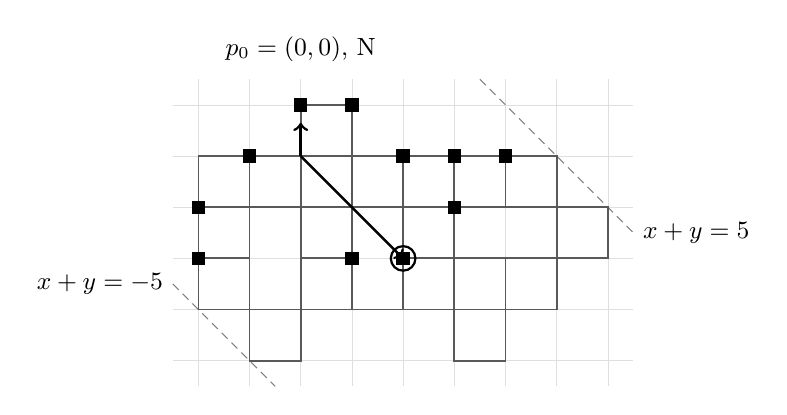
\begin{tikzpicture}[x=0.65cm,y=0.65cm,font=\small]
  % Coordinates represent cell centres, not cell boundaries.
  \draw[gray!25,very thin,step=1] (-2.5,-4.5) grid (6.5,1.5);
  \draw[gray,densely dashed] (-2.5,-2.5) -- (-0.5,-4.5);
  \draw[gray,densely dashed] (3.5,1.5) -- (6.5,-1.5);
  \node[anchor=east] at (-2.5,-2.5) {$x+y=-5$};
  \node[anchor=west] at (6.5,-1.5) {$x+y=5$};
  \draw[black!65,line width=0.65pt] (0,0) -- (1,0) -- (1,-1) -- (0,-1) -- (0,0) -- (-1,0) -- (-1,-1) -- (-2,-1) -- (-2,-2) -- (-1,-2) -- (-1,-3) -- (-2,-3) -- (-2,-2) -- (-1,-2) -- (-1,-1) -- (-2,-1) -- (-2,0) -- (-1,0) -- (-1,-1) -- (-2,-1) -- (-2,-2) -- (-1,-2) -- (-1,-3) -- (0,-3) -- (0,-4) -- (-1,-4) -- (-1,-3) -- (0,-3) -- (0,-2) -- (1,-2) -- (1,-1) -- (0,-1) -- (0,-2) -- (1,-2) -- (1,-3) -- (0,-3) -- (0,-2) -- (1,-2) -- (1,-1) -- (2,-1) -- (2,-2) -- (3,-2) -- (3,-3) -- (2,-3) -- (2,-2) -- (3,-2) -- (3,-1) -- (2,-1) -- (2,-2) -- (3,-2) -- (3,-3) -- (4,-3) -- (4,-4) -- (3,-4) -- (3,-3) -- (4,-3) -- (4,-2) -- (5,-2) -- (5,-3) -- (4,-3) -- (4,-2) -- (3,-2) -- (3,-3) -- (4,-3) -- (4,-2) -- (5,-2) -- (5,-1) -- (6,-1) -- (6,-2) -- (5,-2) -- (5,-1) -- (4,-1) -- (4,0) -- (3,0) -- (3,-1) -- (2,-1) -- (2,0) -- (1,0) -- (1,-1) -- (2,-1) -- (2,0) -- (3,0) -- (3,-1) -- (4,-1) -- (4,0) -- (5,0) -- (5,-1) -- (4,-1) -- (4,0) -- (3,0) -- (3,-1) -- (2,-1) -- (2,0) -- (1,0) -- (1,1) -- (0,1) -- (0,0) -- (-1,0) -- (-1,-1) -- (0,-1) -- (0,-2) -- (1,-2) -- (1,-3) -- (2,-3) -- (2,-2);
  \foreach \x/\y in {-2/-2,-2/-1,-1/0,0/1,1/-2,1/1,2/-2,2/0,3/-1,3/0,4/0}
    \fill[black] (\x-0.13,\y-0.13) rectangle (\x+0.13,\y+0.13);
  \draw[->,line width=1pt] (0,0) -- (0,0.65);
  \node[anchor=south] at (0,1.65) {$p_0=(0,0)$, N};
  \draw[->,line width=0.9pt] (0,0) -- (2,-2);
  \draw[line width=0.8pt] (2,-2) circle (0.24);
  
  
\end{tikzpicture}
\caption{\small The actual $104$ moves and eleven-cell seed. Squares
are initially black; repeated trace edges overlap. The long arrow joins
the north-facing origin to its outlined endpoint and denotes net drift,
not one move. Dashed rails attain labels $x+y=\pm5$, whose difference
is $W=10$, not their Euclidean separation.}\label{fig:witness}
\graphiccredit{Data: A.\ Jillhewar, 2026; diagram: algorithmic rendering with Python and LaTeX/TikZ, 2026.}
\end{figure}

The seed supplied by Theorem~\ref{thm:criterion} is
\[
\{(-2,-2),(-2,-1),(-1,0),(0,1),(1,-2),(1,1),
(2,-2),(2,0),(3,-1),(3,0),(4,0)\}.
\]
The criterion and endpoint decomposition prove indefinite repetition
and $|B_{104n}|=11+12n$. Simulation checks the sampled period boundaries.
This attains Theorem~\ref{thm:width}; minimum growth and highway
uniqueness remain open.
Its $22$ classes are twelve odd and ten even, giving $g=12$. Each
has level range at most two; eleven of eighteen exceptional class--level
combinations begin L and supply the seed cells.

The cross-period chronology example above works through one of these classes explicitly.
The level-gap formula gives minimum seed size $11$ over the $104$
cyclic shifts, attained only at shifts $0,33$ with headings normalised
by quarter-turns. This minimum concerns immediate repetition of this word, excluding
transients and other highways \cite{Repo}.
Shift by $100$ symbols and half-turn the translated pose to face north.
This first-L phase has $d=(-2,2)$ and a thirteen-cell least seed
(\texttt{normalisation\_B} in \path{standard_highway.json} \cite{Repo}).
Alternative wake bases give two fixed cap cells, eleven translating cells
and twelve growing strands: $|B_{104n}|=13+12n$. Its $32$ toggled cells
occupy $21$ signed-field orbits (twelve growing, nine zero-sum), distinct
from its $22$ visited classes.

\section{Exact finite-period searches and verification}
The criterion is an exact acceptance test. A phase of least seed size
starts R and has nonnegative turn prefixes by the seed-phase recurrence,
so this normalisation preserves every realisable candidate. The
through-$32$ baseline fixes only initial R; later engines also enforce
nonnegative prefixes. A length-$k$ prefix rank encodes
$k-1$ binary symbols following R, giving $2^{11}$ ranks for $k=12$,
including pruned prefixes. Accepted leaves restore heading, have nonzero
drift and pass exact coset chronology. Positive-growth pruning uses the
proved zero-growth exclusion.

Chronological completion pruning can be proved directly. If the known
symbols in a class's eventual stable order are $s_1\cdots s_m$, the
minimum insertions for an alternating completion starting R and ending L
are
\[
\begin{aligned}
\mathrm{need}_R&=\mathbf1_{s_1=L}+\#\{i:s_i=s_{i+1}=L\},\\
\mathrm{need}_L&=\#\{i:s_i=s_{i+1}=R\}+\mathbf1_{s_m=R}.
\end{aligned}
\]
Each indicated endpoint or equal-symbol gap requires a distinct insertion;
inserting one opposite symbol in every such gap achieves the bound.
Both needs are zero for an empty word. If an odd final class is allowed,
omit the terminal-L requirement. Summing needs across classes and
comparing with the remaining R/L budget is a sound rejection rule.

Archived residue-theorem-free exhaustive runs exclude every nonzero-drift
period $N\le48$. The period-$48$ run records $41{,}710{,}394{,}384$
nodes and $7{,}446{,}719{,}550$ exact evaluations. Growth-eight runs
at $50,52,54,56,58,60$ cover all $2{,}048$ normalised length-twelve
prefix ranks at each period, with zero accepted words. Thus
\[
N>48\quad\text{for every highway},\qquad
N>60\quad\text{if }g=8.
\]
Periods $50$--$58$ use residue pruning; period $60$ uses a hybrid
endpoint-deficit engine with an audited bounded suffix-reachability
calculation. These exclusions depend on complete rank coverage and exact leaf
acceptance. The recorded engine versions must also match the runs. A partial zero-hit run
proves no complete exclusion; the archived long searches were not rerun.

An independent Python checker agrees through length $18$: $524{,}286$
words, including $172{,}092$ heading-reset nonzero-drift words.
This checks the criterion on the stated range. Longer search completion
requires separate evidence. The Java variants share infrastructure.
Independently structured width checkers reproduce local counts;
\path{aggregate_indep.py} audits period-rank completion. The archived
manifest identifies checkers, period-$60$ engines and outputs \cite{Repo}.
Lean verifies conservation/parity kernels and the width-four rank
argument. The other dynamic reductions and complete growth-four verifier
remain unformalised.

\section{The unresolved growth-eight boundary}
The first unexcluded growth is eight. The density theorem gives
$\|d\|_\infty\le4$, while heading parity and signed residues leave
40 nonzero drifts in ten quarter-turn orbits. Representatives are
\[
(1,-1),\ (2,0),\ (2,-2),\ (1,3),\ (1,-3),\ (3,-3),
\ (4,0),\ (2,4),\ (2,-4),\ (4,-4).
\]
Wake arithmetic and partial-rail or cap arguments restrict subfamilies.
Entire drift orbits remain unexcluded. For $d=(1,-3)$, lifted clocks distinguish physical
returns from quotient returns. The archived upper-cap normal form with
inward multiplicities $(1,2,2)$ is excluded at every width and period
by return-heading or clock contradictions; this does not exclude the
lower orientation \cite{Repo}. All ten orbits retain open cases.
Establishing existence requires a word that passes
Theorem~\ref{thm:criterion}; static wakes and relaxed clocks are
insufficient. Whether a growth-eight highway exists remains open,
as does eventual highway entry from every finite seed. In particular,
$g\ge12$ and universal entry are still unproved.
\clearpage
\pagestyle{empty}
\begin{thebibliography}{99}

\bibitem{BunimovichTroubetzkoy1992}
L.~A. Bunimovich and S.~E. Troubetzkoy.
\newblock Recurrence properties of {L}orentz lattice gas cellular automata.
\newblock \emph{J. Stat. Phys.} \textbf{67} (1992), no.~1--2, 289--302.

\bibitem{Etse2026confined}
K.~R. Etse.
\newblock How long can the escaping ant be confined?
\newblock arXiv:2606.26677 (2026).

\bibitem{GajardoLutfallaRao2024}
A.~Gajardo, V.~H. Lutfalla, and M.~Rao.
\newblock Ants on the highway.
\newblock arXiv:2409.10124 (2024); \emph{Natural Computing} \textbf{24} (2025), 497--509.

\bibitem{GajardoMoreiraGoles2002}
A.~Gajardo, A.~Moreira, and E.~Goles.
\newblock Complexity of {L}angton's ant.
\newblock \emph{Discrete Appl. Math.} \textbf{117} (2002), no.~1--3, 41--50.
\newblock doi:10.1016/S0166-218X(00)00334-6; arXiv:nlin/0306022.

\bibitem{Gajardo2003symbolic}
A.~Gajardo.
\newblock A symbolic projection of {L}angton's ant.
\newblock \emph{Discrete Math. Theor. Comput. Sci. Proc.} AB (DMCS'03)
  (2003), 57--68.
\newblock doi:10.46298/dmtcs.2312.

\bibitem{GaleProppSutnerTroubetzkoy1995}
D.~Gale, J.~Propp, S.~Sutherland, and S.~Troubetzkoy.
\newblock Further travels with my ant.
\newblock \emph{Math. Intelligencer} \textbf{17} (1995), no.~3, 48--56.

\bibitem{Langton1986}
C.~G. Langton.
\newblock Studying artificial life with cellular automata.
\newblock \emph{Physica D} \textbf{22} (1986), no.~1--3, 120--149.
\newblock doi:10.1016/0167-2789(86)90237-X.

\bibitem{Lutfalla2025sideways}
V.~H. Lutfalla.
\newblock Sideways on the highways.
\newblock arXiv:2505.05426 (2025).

\bibitem{Traldi2025interlacement}
L.~Traldi.
\newblock Circuit partitions and signed interlacement in 4-regular graphs.
\newblock \emph{Contrib. Discrete Math.} \textbf{20} (2025), no.~2, 456--480.
\newblock doi:10.55016/ojs/cdm.v20i2.62407; arXiv:1607.04233.

\bibitem{Repo}
A.~Jillhewar. \emph{Langton's Ant Supplementary Materials} (2026).
\newblock Public research repository for \emph{Finite-Support Periodic Highways of Langton's Ant}.
Source manuscripts, research notes, exact search certificates, checker source code
and selected Lean checks; research evidence through 27 September 2026,
with the phase, canonical-wake and lifetime audits of 12 October 2026.
The package manifests identify the released files and the earlier search and strip certificates.
\newblock \url{https://github.com/Atharva12456/langtons-ant-supplementary-materials}.
\end{thebibliography}
\end{document}
